\chapter{Introduction}
\label{chap:intro}

%%%%%%%%%%%%%%%%%%%%%%%%%%%%%%%%%%%%%%
\section{Background}

The ability to understand and predict the manner in which neutrons interact with
matter is at the core of nuclear engineering. These interactions produce heat,
transmute and distort materials, and fission the nuclei of heavy atoms to
create more neutrons. Reactor physicists must understand the distribution and
frequency of these interactions in order to arrange materials in such a
way as to sustain a chain reaction of neutron generations. Properly managed, a
population of neutrons can be used for a wide variety of important functions.
Advanced scientific exploration, radioisotope production for medicine and
industry, high-fidelity imaging, advanced cancer therapies, large-scale heat
generation for electricity production... all are examples of what is possible
with a stable and safe source of neutron production.

\begin{figure}
  \centering
  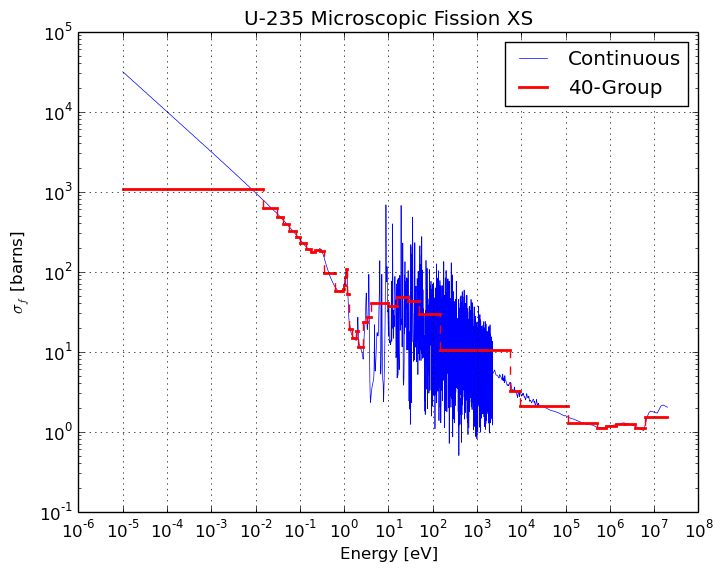
\includegraphics[width=5in]{figures/u235-fission-40-group.png}
  \caption[Uranium-238 capture cross section]{Uranium-235 fission cross section
  showing a typical multi-group discretization for deterministic
  methods.\label{fig:multigroup}}
\end{figure}

\begin{equation}
  \Sigma_{t,g}(\vec{r}) \equiv \frac{\int_{4\pi}d\hat{\Omega}
  \int\limits_{E_g}^{E_{g-1}}dE {\Sigma_{t}(\vec{r},E)
  \psi(\vec{r},\hat{\Omega},E)}}{\int_{4\pi}d\hat{\Omega}
  \int\limits_{E_g}^{E_{g-1}}dE {\psi(\vec{r},\hat{\Omega},E)}}.
\end{equation}